\subsection{Problems}

\noindent {\bf Problem \thesection.\theprob}\stepcounter{prob}

A pump running at $1470 [rpm]$ with $H_{pump}=45-2781 Q^2$ head delivers water into a pipeline with $H_{pipe}=20+1125Q^2$. Calculate the required revolution number for the reduced flow rate $Q'=0.05 [m^3/s]$. 

\vspace{0.5cm}
\begin{tabular}{cc}
    \begin{minipage}{9cm}
	\begin{center}
	    \resizebox{9cm}{!}{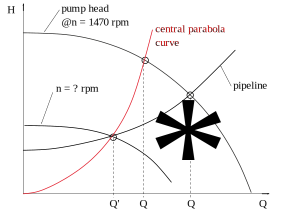
\includegraphics{Problem_solving/figs/PS_OperatingPoint_Affinity.png}}\\
	\end{center}
    \end{minipage}
& 

\begin{minipage}{6cm}

\noindent Solution: 

\begin{itemize}
\item The ac\-tual wor\-king point is given by the so\-lu\-tion of $H_{pump}=H_{pipe}$, which gives $Q=0.08 [m^3/s]$ and $H=27.2[m]$.
\item Affinity states that while varying the revolutionary speed, $H/n^2$ and $Q/n$ remain constant. Thus, also $H/Q^2$ remains constant, let's denote this constant by $a$. So, while varying the revolutionary speed, the working point moves along the \emph{central parabola} (see figure), given by $H_{ap}=a\,Q^2$.
\end{itemize}
\end{minipage}
\end{tabular}

However, as $Q'$ is given and we also know that this point has to be located on the pipeline characteristic, we know that $H'= 20+1125 \cdot 0.05^2=22.81[m]$. Thus, the parameter of the affine parabola is $a=H'/Q'^2=9125$. 

$Q^*$ is given by the intersection of the affine parabola and the original pump characteristic: $H_{ap}(Q^*)=H_{pump}(Q^*)$, which gives $Q^*=0.06148[m^3/s]$ with $H^*=34.5[m]$.

Now we can employ affinity between $Q^*$ and $Q'$:

\begin{equation*}
n'=n^*\frac{Q'}{Q^*}=1470\times \frac{0.05}{0.06148}=1195.5 [rpm] 
\end{equation*}

and just for checking the calculation

\begin{equation*}
H'=H^* \left(\frac{n'}{n^*} \right)^2=34.5\times \frac{1195.5^2}{1470^2}=22.81 [m].
\end{equation*}

%%%%%%%%%%%%%%%%%%%%%%%%%%%%%%%%%%%%%%%%%%%%%%%%%%%%%%%%%%%%%%%%%%%%

\vspace{1cm}
\noindent {\bf Problem \thesection.\theprob}\stepcounter{prob}

Solve the previous control problem (pump: $H_{pump}=45-2781 Q^2$, pipeline: $H_{pipe}=20+1125Q^2$, desired flow rate: $Q'=0.05 [m^3/s]$) using a throttle at the pressure side of the pump and also with a bypass line. Compare the resulting operations in terms of power loss!

\begin{figure}[!ht]
\centering
\includegraphics[width=0.7\textwidth]{Problem_solving/figs/PS_Control1.png}
\end{figure}

%%%%%%%%%%%%%%%%%%%%%%%%%%%%%%%%%%%%%%%%%%%%%%%%%%%%%%%%%%%%%%%%%%%%%%

\vspace{1cm}
\noindent {\bf Problem \thesection.\theprob}\stepcounter{prob}

A pump, whose characteristic curve is given by $H_{pump}=70-90000[s^2/m^5]Q^2$, works together with two parallel pipes. The main pipe is given by $H_1=30+100000[s^2/m^5]Q^2$. Calculate the head-flow relationship $H_2(Q)$ of the side pipe, whose opening results in a flow rate of $480[l/min]$ in the main pipe. The static head of the second side pipe is $25[m]$.

\noindent Solution: 

\begin{itemize}
\item Head of the main pipe at the prescribed flow rate: $Q_1 = 480[l/min]=0.008[m^3/s] \quad \rightarrow \quad H_1(Q_1)=36.4[m]$
%
\item The head is the same, so the flow rate of the pump is
 $H_p(Q_p)= H_1(Q_1) \quad \rightarrow \quad Q_p=\sqrt{\frac{70-36.4}{90000}}=0.0193[m^3/s]$
%
\item Thus, the flow rate on the side pipe is $Q_2=Q_p-Q_1=0.0193-0.008=0.0113[m^3/s]$
%
\item The actual characteristic of the side pipe: $H_2(Q_2)=25+aQ_2^2=36.4[m] \quad \rightarrow \quad a=\frac{36.4-25}{0.0113^2}=89279$
%
\item The solution is $H_2(Q_2)=25+89279 Q^2$.
\end{itemize}

%%%%%%%%%%%%%%%%%%%%%%%%%%%%%%%%%%%%%%%%%%%%%%%%%%%%

\vspace{1cm}
\noindent {\bf Problem \thesection.\theprob}\stepcounter{prob}

Pumps $I$ and $II$ feed pipes $1$ and $2$ shown in the figure below. Their characteristics are:
\begin{eqnarray}
	&& H_I = 45m-24900s^2/m^5Q^2 \nonumber \\
	&& H_{II} = 35m-32200s^2/m^5Q^2 \nonumber \\
	&& H_1 = 10m+4730s^2/m^5Q^2 \nonumber \\
	&& H_2 = 15m+8000s^2/m^5Q^2\nonumber
\end{eqnarray}
Find the flow rates and heads if valve $"V"$ is closed, and if it it opened. 
0.023054084926172
% (Solution: closed: $H=34.46~\mathrm{m},~Q=0.02578~\frac{\mathrm{m^3}}{\mathrm{s}}$; open:  $H=25.18\mathrm{m},~Q=0.03567~\frac{\mathrm{m^3}}{\mathrm{s}}$)
(Solution: closed: $H=31.766~\mathrm{m},~Q=0.02305~\frac{\mathrm{m^3}}{\mathrm{s}}$; open:  $H=25.18\mathrm{m},~Q=0.03567~\frac{\mathrm{m^3}}{\mathrm{s}}$)

\begin{figure}[!ht]
\centering
\includegraphics{Problem_solving/figs/PS_Control_Pumps.png}
\end{figure}

%%%%%%%%%%%%%%%%%%%%%%%%%%%%%%%%%%%%%%%%%%%%%%%%%%%%%%%%%%%%%%%%%%%%%%%%%%
\vspace{1cm}
\noindent {\bf Problem \thesection.\theprob}\stepcounter{prob}

Two pumps, $H_1=70m-50000s^2/m^5Q^2$ and $H_2=80m-50000s^2/m^5Q^2$ can be coupled parallel or in series. Which arrangement will deliver more liquid through the pipe $H_p=20m+25000s^2/m^5Q^2$? (Solution: in series: $Q=0.03224~\frac{\mathrm{m^3}}{\mathrm{s}},~H=46~\mathrm{m}$; in parallel: $Q=0.03818~\frac{\mathrm{m^3}}{\mathrm{s}},~H=56.44~\mathrm{m}$)

%%%%%%%%%%%%%%%%%%%%%%%%%%%%%%%%%%%%%%%%%%%%%%%%%%%%

\vspace{1cm}
\noindent {\bf Problem \thesection.\theprob}\stepcounter{prob}

Pump S, with the characteristitc curve $H_S=37-0.159Q^2$, is feeding an irrigation system consisting of parallel pipes. The units are $Q[m3/h]$ and $H[m]$. Each pipe contains at its end a sprinkler. The pipes are $20m$ long, their inner diameter is $25mm$, the friction coefficient is $0.03$. The sprinklers discharge $4 m^3/h$ water at $2 bar$ overpressure, their characteristics can be written as $H_{spr}=K_{spr}Q^2$. 

\begin{itemize}
\item Draw the sketch of the irrigation system with 3 parallel pipes!
\item How much water is discharged if only one pipe is in operation?
\item How many parallel pipes can be fed if the overpressure before the sprinklers must be $2 bar$? 
\end{itemize}

(Solution: single pipe: $Q_1 = 4.5~\frac{\mathrm{m^3}}{\mathrm{h}}$, $H=33.7~\mathrm{m}$; the pump can supply 2 pipes only)

%%%%%%%%%%%%%%%%%%%%%%%%%%%%%%%%%%%%%%%%%%%%%%%%%%%%

\vspace{1cm}
\noindent {\bf Problem \thesection.\theprob}\stepcounter{prob}

The characteristics of a pump supplying a small village with water is $H_p=70-330Q^2$. The village network is modeled by the curve $H_{cd}=25+30Q^2$ during the day while the night operation can be described by $H_{cn}=25+750Q^2$. A high water tower is attached to the delivery tube of the pump, its characteristics is $H_T=40-55|Q|Q $. Here $Q$ is positive if water flows down from the tower. The units in the formulae are [Q] = m3/s; [H] = m. Draw a sketch of the water system. Find the flow rates of the pump, village and tower both for day and night operation. Find the head of the pump both for day and night! Use a millimeter paper to draw the charasteristics curves! (Solutions: $Q_{pump}=0.33m^3/s$ and $0.29m^3/s$; $Q_{village}=0.6m^3/s$ and $0.15m^3/s$; $Q_{tower}=0.275m^3/s$ and $-0.14m^3/s$. $H_{pump}=36m$ and $41m$.)
%%%%%%%%%%%%%%%%%%%%%%%%%%%%%%%%%%%%%%%%%%%%%%%%%%%%

\vspace{1cm}
\noindent {\bf Problem \thesection.\theprob}\stepcounter{prob}

How much water is delivered by the pump $H_p=70-45000Q^2$ through the pipe system $H_s = 20+20000Q^2$ ? The flow rate must be reduced to $0.015 m^3/s$. This can be done either by throttling control or by using a by-pass control. Draw the pump-pipe-valve arrangements for both cases. How large is the hydraulic loss in the valves in the first and in the second case? The power consumption of the pump is $P_{input} = 9.4+240Q-50000Q^2$. How large is the specific energy consumption $f$ in the two cases? The units in the formulae are: $[m], [m^3/s], [kW]$. (Solution: $Q= 0.0277~\frac{\mathrm{m^3}}{\mathrm{s}}$, $P_{throttle}' = 5.2~\mathrm{kW}$, $P_{bypass}'=4.0~\mathrm{kW}$, $\mathrm{SEC}=0.237~\frac{\mathrm{kWh}}{\mathrm{m^3}}$ and $\mathrm{SEC}=0.285~\frac{\mathrm{kWh}}{\mathrm{m^3}}$, respectively.)

